\documentclass[11pt,spanish,a4paper]{article}
% Versión 1.er cuat 2021 Víctor Bettachini < bettachini@df.uba.ar >

% Versión 1.er cuat 2021 Víctor Bettachini < bettachini@df.uba.ar >

\usepackage[T1]{fontenc}
\usepackage[utf8]{inputenc}

\usepackage[spanish, es-tabla]{babel}
\def\spanishoptions{argentina} % Was macht dass?
% \usepackage{babelbib}
% \selectbiblanguage{spanish}
% \addto\shorthandsspanish{\spanishdeactivate{~<>}}

\usepackage{graphicx}
\graphicspath{{./figuras/}{../LaTeX/}}
% \usepackage{float}

\usepackage[arrowdel]{physics}
\newcommand{\pvec}[1]{\vec{#1}\mkern2mu\vphantom{#1}}
% \usepackage{units}
\usepackage[separate-uncertainty=true, multi-part-units=single, locale=FR]{siunitx}
\usepackage{isotope} % $\isotope[A][Z]{X}\to\isotope[A-4][Z-2]{Y}+\isotope[4][2]{\alpha}

\usepackage{tasks}
\usepackage[inline]{enumitem}
% \usepackage{enumerate}

\usepackage{hyperref}

% \usepackage{amsmath}
% \usepackage{amstext}
\usepackage{amssymb}

\usepackage{tikz}
\usepackage{tikz-dimline}
\usetikzlibrary{calc}
% \usetikzlibrary{math}
\usetikzlibrary{arrows.meta}
\usetikzlibrary{snakes}
\usetikzlibrary{decorations}
\usetikzlibrary{decorations.pathmorphing}
\usetikzlibrary{patterns}

% \usepackage[hmargin=1cm, vmargin=1cm, includeheadfoot]{geometry}
\usepackage[hmargin=1cm,vmargin=3cm, top= 0.75cm,nohead]{geometry}
% \voffset-3.5cm
% \hoffset-3cm
% \setlength{\textwidth}{17.5cm}
% \setlength{\textheight}{27cm}

\usepackage{lastpage}
\usepackage{fancyhdr}
\pagestyle{fancyplain}
\fancyhf{}
% \fancyhead{}
\setlength\headheight{28.7pt} 
\fancyhead[LE, LO]{\textbf{Física 2} (Físicos) }
% \lhead{\textbf{Física 2} (Físicos) }
\fancyhead[RE, RO]{\href{https://df.uba.ar/es/}{$\vcenter{\hbox{\includegraphics[height=1cm]{sin_texto.pdf}}}$}}
% \rhead{$\vcenter{\hbox{\includegraphics[height=1cm]{sin_texto.jpg}}}$}
% \rhead{\includegraphics[height=1cm]{sin_texto.jpg}}
% \rhead{\textcopyright {\tt DF, FCEyN, UBA}}
\fancyfoot{\href{https://creativecommons.org/licenses/by-sa/4.0/deed.es/}{$\vcenter{\hbox{\includegraphics[height=0.4cm]{cc-by-sa.pdf}}}$} \href{https://df.uba.ar/es/}{DF, FCEyN, UBA}}
% \fancyfoot{$\vcenter{\hbox{\includegraphics[height=0.4cm]{cc-by-sa.pdf}}}$ DF, FCEyN, UBA}
% \fancyfoot{{\tiny \textcopyright DF, FCEyN, UBA}}
\fancyfoot[C]{ {\tiny Actualizado al \today} }
\fancyfoot[RO, LE]{Pág. \thepage/\pageref{LastPage}}
\renewcommand{\headrulewidth}{0pt}
\renewcommand{\footrulewidth}{0pt}


\begin{document}
\begin{center}
\textbf{Física 2} (Físicos) \hfill \textcopyright {\tt DF, FCEyN, UBA}\\
	\textsc{\LARGE Ondas viajeras y estacionarias}
\end{center}

Los ejercicios con (*) son opcionales.

\begin{enumerate}


\subsection*{Parámetros de una onda viajera}

\item Verifique si las siguientes expresiones matemáticas cumplen la ecuación
de las ondas unidimensional.
Grafique las funciones dadas.
\begin{tasks}(3)
	\task $\Psi(x,t)= A \operatorname{e}^{- \lambda ( x - v t)^2 }$
	\task $\Psi(x,t)= \beta ( x + v t )$
	\task $\Psi(x,t)= A \sen{\left[ k (x - v t) \right] }$
	\task $\Psi(x,t)= B \sen^2{ \left( k x -\omega t \right) }$
	\task $\Psi(x,t)= C \cos{(k x)} \sen{ \left( \omega t \right) }$
	\task $\Psi(x,t)= D \operatorname{e}^{i ( k x - \omega t ) }$
\end{tasks}


\item La ecuación de una onda transversal en una cuerda está dada por: $y(x,t) = \SI{0.1}{\metre} \sen{ \left( x \SI{\pi}{\per\metre} - t \SI{4 \pi}{\per\second} \right) }$.
Determine para la onda que se propaga en ella:
\begin{tasks}(2)
	\task amplitud,
	\task frecuencia de vibración, y
	\task velocidad de propagación.
	\task Y en $x = \SI{2}{\metre}$ y $ t = \SI{1}{\second}$, desplazamiento, velocidad y la aceleración de la cuerda.
\end{tasks}


\item La frecuencia angular y número de onda de una onda transversal que se propaga en $\hat{x}$ es $\omega= \SI{10}{\per\second}$ y $k = \SI{100}{\per\metre}$.
En $x_1 = \SI{1}{\kilo\metre}$ y $t_1 = \SI{1}{\second}$ tiene por fase $\phi = \frac{3 \pi}{2}$.
\begin{tasks}
	\task ¿Cuál es la fase en ese mismo punto para $t = 0$?
	\task Considerando que $\phi(x,t) = k x - \omega t+ \phi_0$, ¿cuánto vale $\phi_0$?
	\task ¿A qué velocidad se propaga la onda?
	\task ¿En que tiempo el frente de onda arriba a un $x_2 = 2 x_1$?
\end{tasks}


\item Una cuerda con densidad lineal $\mu = \SI{0.005}{\kilo\gram\over\metre}$ se tensa aplicando una fuerza de \SI{0.25}{\newton}.
El extremo izquierdo se mueve hacia arriba y hacia abajo con un movimiento armónico simple de período \SI{0.5}{\second} y amplitud \SI{0.2}{\metre} mientras se mantiene la tensión constante.
Encontrar:
\begin{enumerate}
	\item La velocidad de la onda generada en la cuerda, la frecuencia y la longitud de onda.
	\item La expresión matemática para el desplazamiento: $y(x,t)$.
	\item La energía cinética media por unidad de longitud, de una partícula del medio.
	\item La energía potencial media por unidad de longitud, de una partícula.
\end{enumerate}


\subsection*{Estacionarias en una cuerda como superposición de viajeras}

\item 
\begin{minipage}[t][2cm]{0.6\textwidth}
Una cuerda de longitud $L = \SI{0.6}{\metre}$, fija en sus dos extremos, oscila en uno de sus modos normales.
La velocidad de propagación de las ondas en dicha cuerda es \(v = \SI{80}{\metre\over\second}\).
En el momento que presenta su máxima amplitud pico a pico esta es de \SI{8}{\milli\metre}.
\end{minipage}
\begin{minipage}[c][1.5cm][t]{0.34\textwidth}
	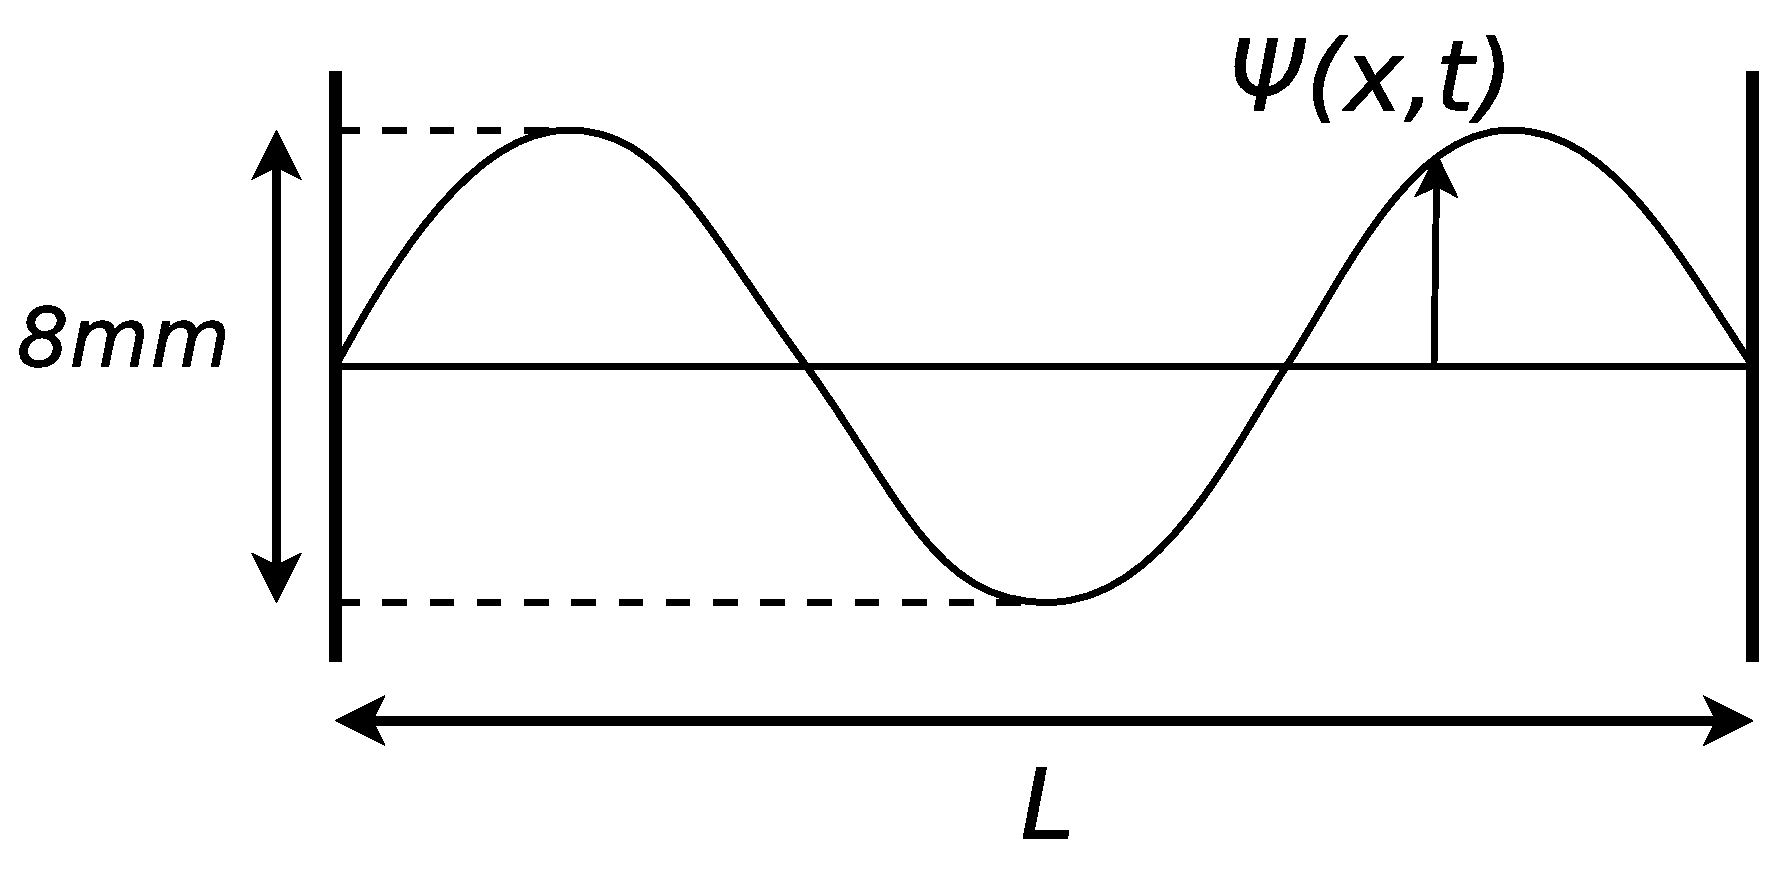
\includegraphics[width=\textwidth]{ej1-32}
\end{minipage}
\begin{enumerate}
	\item Escribir $\Psi(x,t)$, sabiendo que a $\Psi(x,0) = 0\;\forall x$, y que $\dot{\Psi}(L/2,0) > 0$.
	\item Hallar las ondas viajeras $\Psi_{1,2}$ tales que $\Psi(x,t)$ sea una combinación lineal de estas.
\end{enumerate}


\item 
\begin{minipage}[t][2.6cm]{0.6\textwidth}
Una cuerda de longitud $L = \SI{1}{\metre}$, con un extremo fijo y uno libre, oscila en uno de sus modos normales.
La velocidad de propagación de las ondas en dicha cuerda es \(v= \SI{80}{\metre\over\second}\).
En \(t = 0\) presenta su máxima amplitud pico a pico de \SI{8}{\milli\metre}, siendo $\Psi(L,0) > 0$.
\end{minipage}
\begin{minipage}[c][0.4cm][t]{0.34\textwidth}
	\includegraphics[width=\textwidth]{ej1-33}
\end{minipage}
\begin{enumerate}
	\item Resolver, para esta situación, todo lo pedido en el problema anterior. 
	\item Si ahora la cuerda está oscilando en un modo normal arbitrario $n$, con las mismas condiciones iniciales dadas arriba, repetir (a) (expresar en función de $n$).
\end{enumerate}



\subsection*{Propagación en medios no dispersivos}

\item
\begin{minipage}[t][2.6cm]{0.4\textwidth}
\fussy
Una perturbación se propaga en una cuerda infinita con velocidad $v$.
Las figuras la muestran en $t =0$ y $t = \SI{4}{\second}$.
Determine $v$ y $\psi(x,t)$.
\end{minipage}
\begin{minipage}[c][1.1cm][t]{0.54\textwidth}
	\begin{tikzpicture}
		\tikzmath{
			\Dt= 2;
			\t0= 1;
			\haute= 1;
			\xmin= -1;
			\xmax= 6.5;
			\ymin= 0;
			\ymax= 2;
		}
		\coordinate (quiebreInferior) at (\t0/2,0);
		\coordinate (quiebreSuperior) at ({(\t0+\Dt)/2},\haute);
		\coordinate (quiebreSuperiorDebajo) at ({(\t0+\Dt)/2},0);
		\draw [-Latex] (\xmin/2,0) -- (\xmax/2,0) node [anchor=north] {\(x\) [m]};	% eje x
		\draw [Latex-](0,\ymax) node [anchor=west] {\( \psi(x,0) \)} -- (0,\ymin) node [anchor=north] {\(0\)};	% eje y
		\draw [ultra thick] (\xmin/2,0) -- (quiebreInferior) node [anchor = north] {\t0} -- (quiebreSuperior) -- (quiebreSuperiorDebajo) node [anchor = north] {\( 3 \)} -- (\xmax/2-0.15,0);	% cuerda
		% \draw [ultra thick] (\xmin/2,0) -- (quiebreInferior) node [anchor = north] {\t0} -- (quiebreSuperior) node [anchor = south west] {\(t=0\)}-- (quiebreSuperiorDebajo) node [anchor = north] {3} -- (\xmax/2-0.15,0);	% cuerda
		\draw [thin, dashed] (0,\haute) node [anchor=east] {\( 1 \)} -- (quiebreSuperior);
	\end{tikzpicture}
	\quad
	\begin{tikzpicture}
		\tikzmath{
			\Dt= 2;
			\t0= 1;
			\haute= 1;
			\xmin= -1;
			\xmax= 6.5;
			\ymin= 0;
			\ymax= 2;
		}
		\coordinate (quiebreInferior) at ({(\t0+\Dt)/2},0);
		\coordinate (quiebreSuperior) at ({(\t0+\Dt+\Dt)/2},\haute);
		\coordinate (quiebreSuperiorDebajo) at ({(\t0+\Dt+\Dt)/2},0);
		\draw [-Latex] (\xmin/2,0) -- (\xmax/2,0) node [anchor=north] {\(x\) [m]};	% eje x
		\draw [Latex-](0,\ymax) node [anchor=west] {\( \psi(x,4 s) \)} -- (0,\ymin) node [anchor=north] {\(0\)};	% eje y
		\draw [ultra thick] (\xmin/2,0) -- (quiebreInferior) node [anchor = north] {\( 3 \)} -- (quiebreSuperior) -- (quiebreSuperiorDebajo) node [anchor = north] {\( 5 \)} -- (\xmax/2-0.15,0);	% cuerda
		\draw [thin, dashed] (0,\haute) node [anchor=east] {\( 1 \)} -- (quiebreSuperior);
	\end{tikzpicture}
\end{minipage}
	Suponga ahora que conoce que $v = \SI{100}{\metre\over\second}$ y vé que la cuerda fue soltada desde el reposo con la deformación vista en $t=0$.
\begin{enumerate}
	\item Halle las componentes de la perturbación que se propagan a izquierda y derecha que conforman $\psi(x,t) = \psi_\text{derecha} (x - v t ) + \psi_\text{izquierda} ( x + v t )$.
	% Dé explícitamente (en cada intervalo de interés) la expresión de $\psi(x,t)$.
	\item Comparé esta situación con la anterior.
\end{enumerate}



\item (*) Ambos extremos de una cuerda de densidad $\mu$ están fijos sometiéndola a una tensión $T$.
A $t=0$ se la suelta con $h \ll L$ desde
$
\psi(x,0)=\begin{cases}
0 & \mbox{si }0<x<a\\
h\frac{x-a}{L/2-a} & \mbox{si }a<x<L/2\\
h\frac{L-a-x}{L/2-a} & \mbox{si }L/2<x<L-a\\
0 & \mbox{si }L-a<x<L .
\end{cases}
$
\begin{enumerate}
	\item Hallar $\psi(x,t)$ y demostrar que siempre es posible escribir esta solución como una superposición de una onda que se propaga hacia la derecha y una que se propaga hacia la izquierda.
	\item Hacer un esquema cualitativo del movimiento de la cuerda para los instantes $t_n = \frac{n}{8} \frac{L}{v}$, donde $v$ es la velocidad de propagación de las ondas en la cuerda y $n$ es un número natural.
\end{enumerate}


\item 
\begin{minipage}[t][1.5cm]{0.7\textwidth}
(*) En un gas, a $t=0$, se produce la perturbación indicada en la figura.
Conociendo la $v_\text{sonido}$, $\rho_{1}$, $\rho_{0}$ tales que $(\rho_{1}-\rho_{0})/\rho_{0}\ll1$ y que en ese momento el gas estaba en reposo, calcule $\rho(x,t)$.
\end{minipage}
\begin{minipage}[c][1.6cm][t]{0.2\textwidth}
	\begin{tikzpicture}
		\tikzmath{
			\rrho0= 0.3;
			\rrho1= 0.8;
			\xmax= 2;
			\xmin= -\xmax;
			\ymax= 1.5;
			\ymin= 0;
		}
		\draw [-Latex] (\xmin,0) -- (\xmax,0) node [anchor=north] {\( x \)};	% eje x
		\draw [Latex-](0,\ymax) node [anchor=west] {\( \rho(x,0) \)} -- (0,\ymin) node [anchor=north] {\(0\)};	% eje y
		\draw [ultra thick] (0,\rrho0) node [anchor = east] {\( \rho_0 \)} -- (\xmax,\rrho0);
		\draw [ultra thick] (0,\rrho1) node [anchor = west] {\( \rho_1 \)} -- (\xmin,\rrho1);
	\end{tikzpicture}
	% \includegraphics[width=\textwidth]{ej2-5}
\end{minipage}


\item 
\begin{minipage}[t][2.1cm]{0.6\textwidth}
Dos cuerdas semi-infinitas de distinta densidad lineal de masa, $\rho_\text{izq}$ y $\rho_\text{der}$, están unidas en un punto y sometidas a una tensión $T_0$.
Sobre la primera se propaga hacia la derecha la perturbación que muestra la figura.
Se conocen $\rho_\text{izq}$, $\rho_\text{der}$, $T_0$, $\Delta x$ y $h$, y se considera que los medios son no dispersivos.
\end{minipage}
\begin{minipage}[c][0.4cm][t]{0.34\textwidth}
	\begin{tikzpicture}
		\tikzmath{
			\Deltax = 1;
			\x0 = -1;
			\haute = 1;
			\xmin = -2.5;
			\xmax = -\xmin;
			\ymin = 0;
			\ymax = 2;
		}
		\coordinate (quiebreIzq) at ({(\x0-\Deltax/2)},0);
		\coordinate (quiebreSuperior) at ({\x0},\haute);
		\coordinate (quiebreDer) at ({(\x0+\Deltax/2)},0);
		\draw [-Latex, thin] (\xmin,0) -- (\xmax,0) node [anchor=north] {\(x\) [m]};	% eje x
		\draw [Latex-, thin](0,\ymax) node [anchor=west] {\( \psi(x,0) \)} -- (0,\ymin) node [anchor=north] {\(0\)};	% eje y
		\draw [ultra thick] (\xmin+0.3,0) -- (quiebreIzq) -- (quiebreSuperior) -- (quiebreDer) -- (0,0);	% cuerda izq
		\draw [ultra thick, gray] (0,0) -- ({\xmax-.3},0);	% cuerda der
		\draw [thin, dashed] (0,\haute) node [anchor = west] {\( h \)} -- (quiebreSuperior);
		\dimline [label style= {above=0}, extension start length=-0.6, extension end length=-0.6]{(-1.5,-.6)}{(-0.5,-.6)}{\( \Delta x \)};
	\end{tikzpicture}
% 	\includegraphics[width=\textwidth]{ej2-20}
\end{minipage}
\begin{enumerate}
	\item Hallar el desplazamiento $\psi(x,t)$.
	\item Explique cualitativamente como cambian estos resultados si el medio es dispersivo.
\end{enumerate}





\end{enumerate}

\end{document}
